\section{Problem 3}

\subsection{Introduction}
This report details the implementation of dimensionality reduction techniques using Principal Component Analysis (PCA) and t-distributed Stochastic Neighbor Embedding (t-SNE) on the MNIST dataset and another dataset referred to as the e6 dataset. These techniques are crucial in exploratory data analysis, especially in high-dimensional datasets, allowing for better visualization and interpretation.

\subsection{Data Loading and Preprocessing}
The code begins by loading the MNIST test dataset and the e6 dataset. For the MNIST dataset, the features are separated from the labels. The e6 dataset undergoes additional preprocessing steps to handle missing values and convert date formats.

\subsubsection{Loading the MNIST Dataset}
The following code snippet loads the MNIST dataset:
\begin{lstlisting}[language=Python]
mnist_test = pd.read_csv('mnist_test.csv')
X = mnist_test.drop('label', axis=1)
y = mnist_test['label']
\end{lstlisting}

\subsubsection{Loading the e6 Dataset}
The e6 dataset is loaded and preprocessed to manage missing values and convert the datetime column:
\begin{lstlisting}[language=Python]
e6_data = pd.read_csv('e6-Run2-June22-subset-100-cols.csv')
e6_data.replace('#REF!', np.nan, inplace=True)
e6_data.iloc[:, 0] = pd.to_datetime(e6_data.iloc[:, 0], format='%d-%m-%Y')
\end{lstlisting}

\subsection{Standardization}
Standardization is a critical step in data preprocessing to ensure that each feature contributes equally to the analysis. This is achieved using the \texttt{StandardScaler} class from the \texttt{sklearn.preprocessing} module.

\begin{lstlisting}[language=Python]
scaler = StandardScaler()
X_scaled = scaler.fit_transform(X)
\end{lstlisting}

\subsection{Dimensionality Reduction}
Two dimensionality reduction techniques are applied to the datasets: PCA and t-SNE.

\subsubsection{PCA Implementation}
PCA is used to reduce the dimensionality of the MNIST dataset while analyzing the explained variance. The cumulative explained variance is computed and visualized to identify the optimal number of components.

\begin{lstlisting}[language=Python]
pca = PCA()
X_pca = pca.fit_transform(X_scaled)
explained_variance_ratio = pca.explained_variance_ratio_
cumulative_variance = np.cumsum(explained_variance_ratio)
\end{lstlisting}

The elbow diagram illustrating the cumulative explained variance is shown in Figure \ref{fig:elbow_diagram}.

\begin{figure}[H]
    \centering
    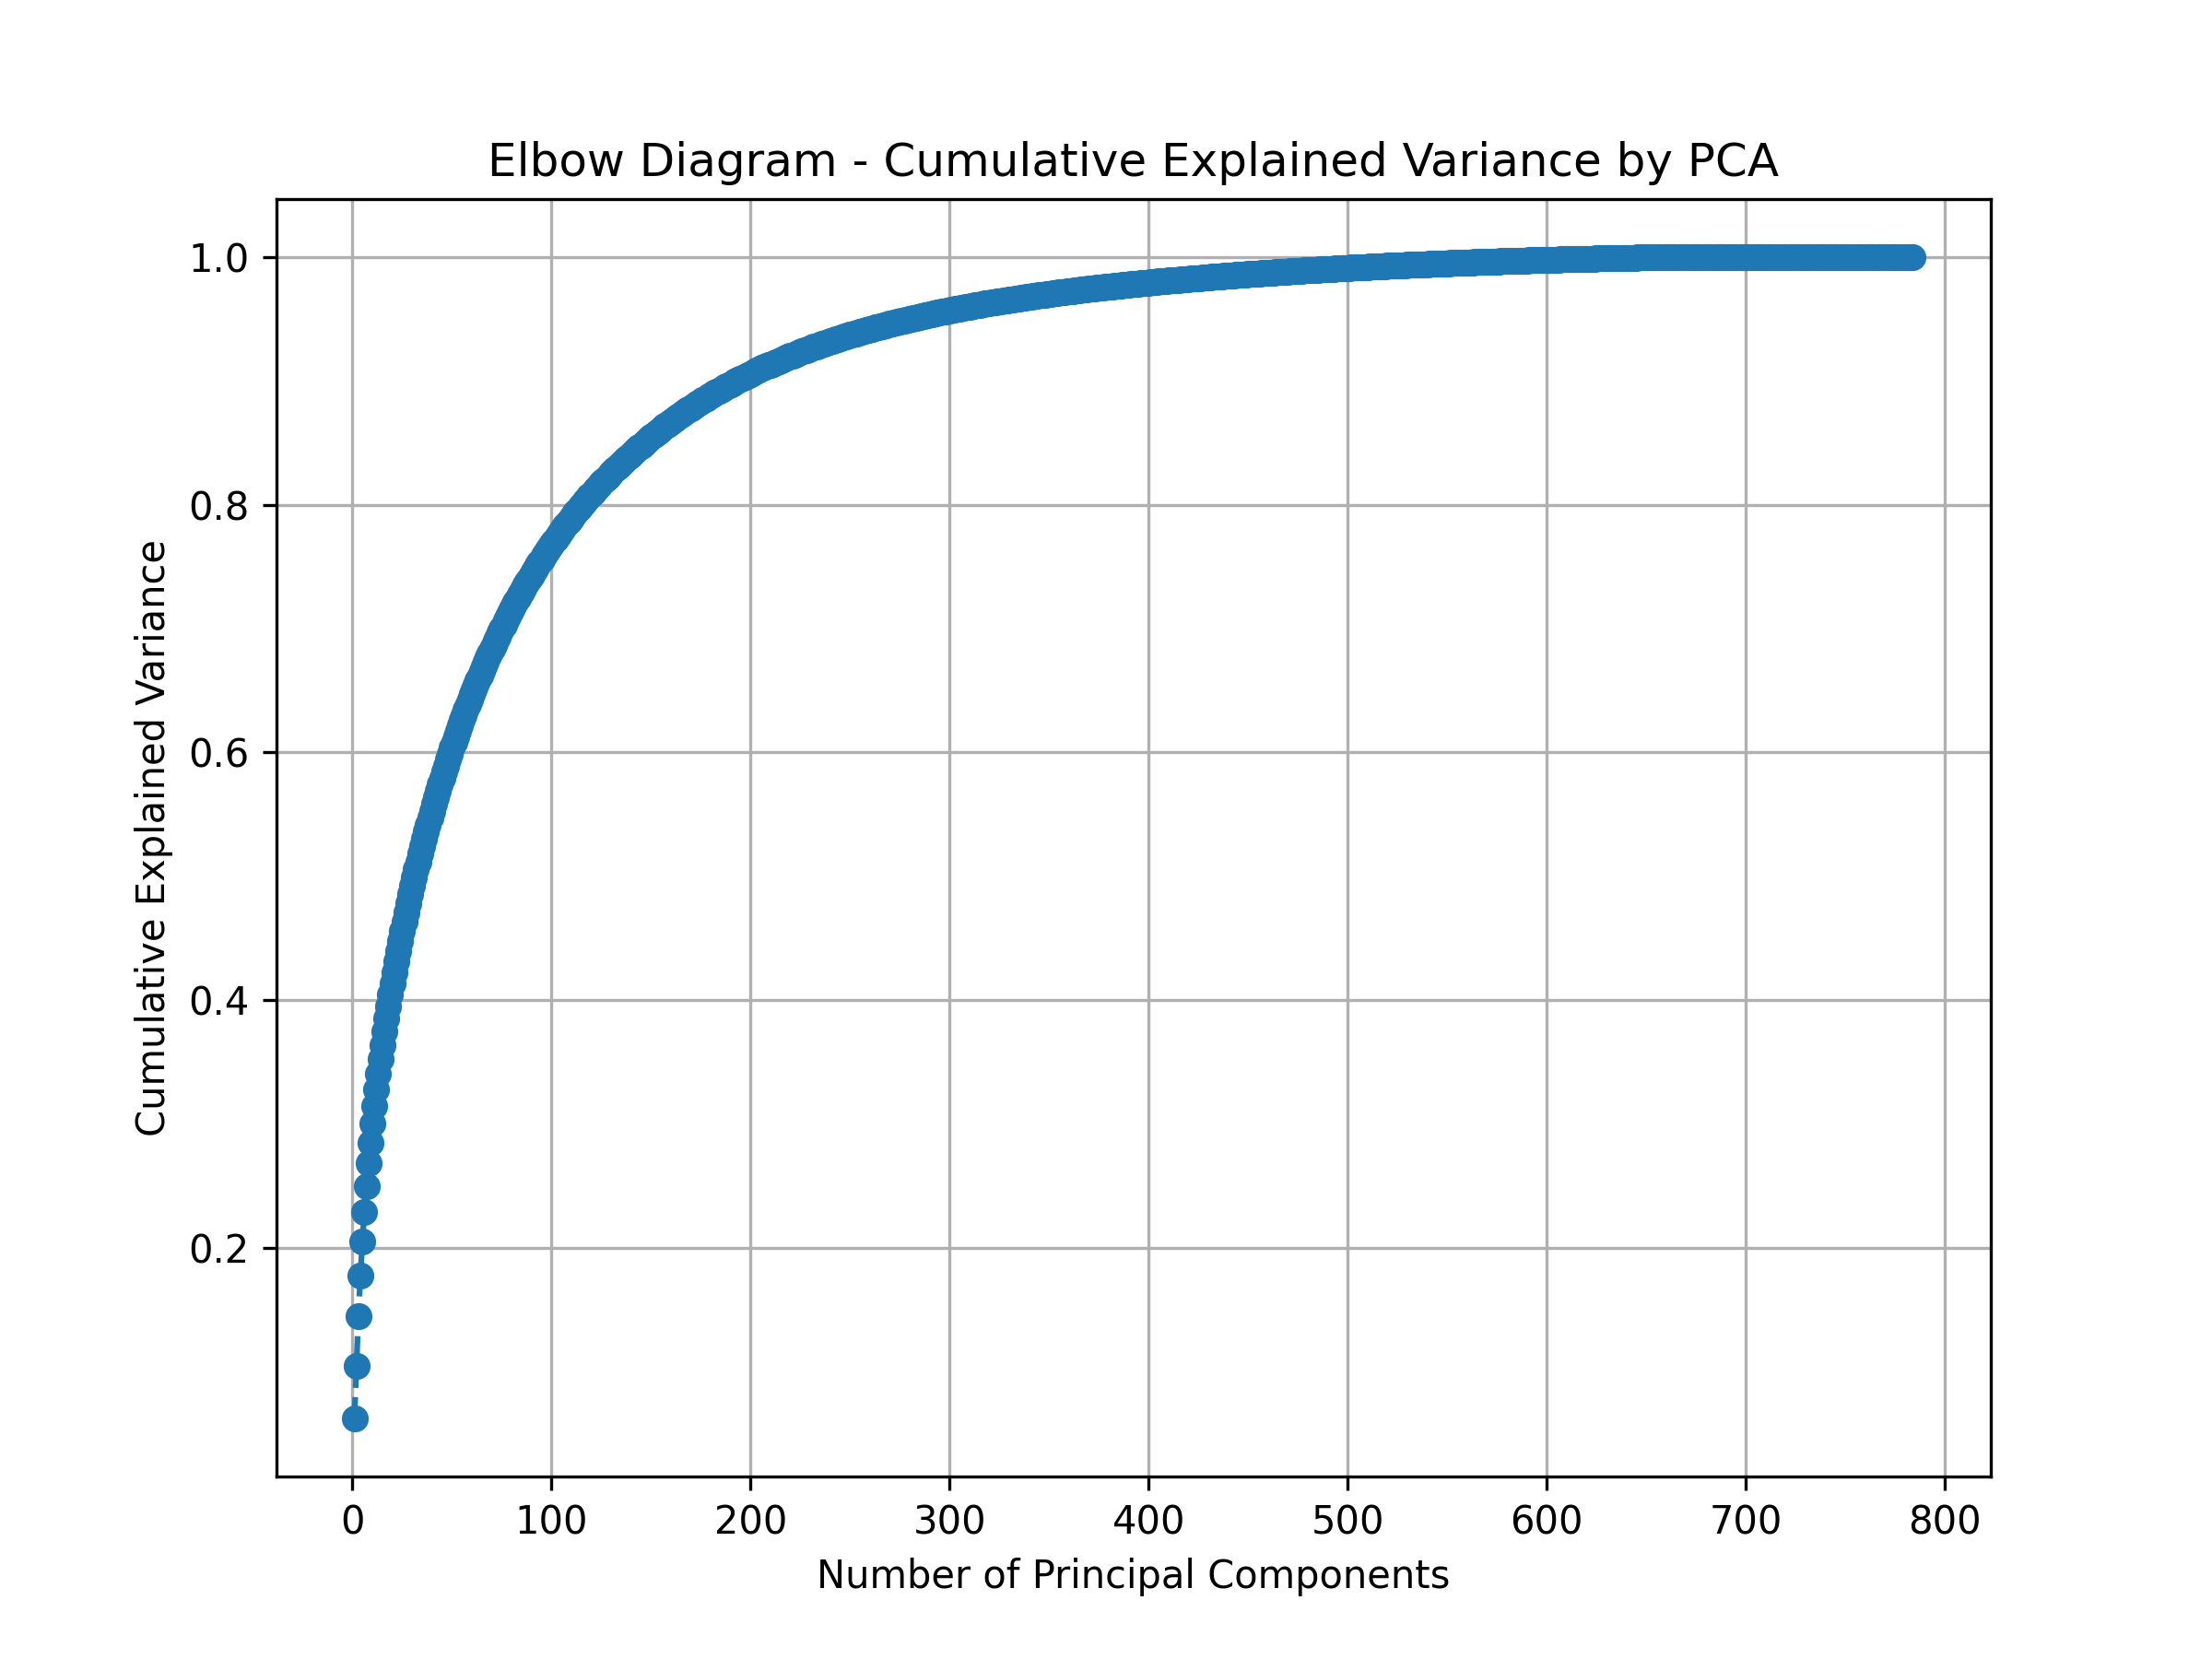
\includegraphics[width=0.6\textwidth]{Images/P3-elbow_diagram.png}
    \caption{Elbow Diagram - Cumulative Explained Variance by PCA}
    \label{fig:elbow_diagram}
\end{figure}

The first two principal components are visualized in the scatter plot in Figure \ref{fig:pca_scatter_plot}.

\begin{figure}[H]
    \centering
    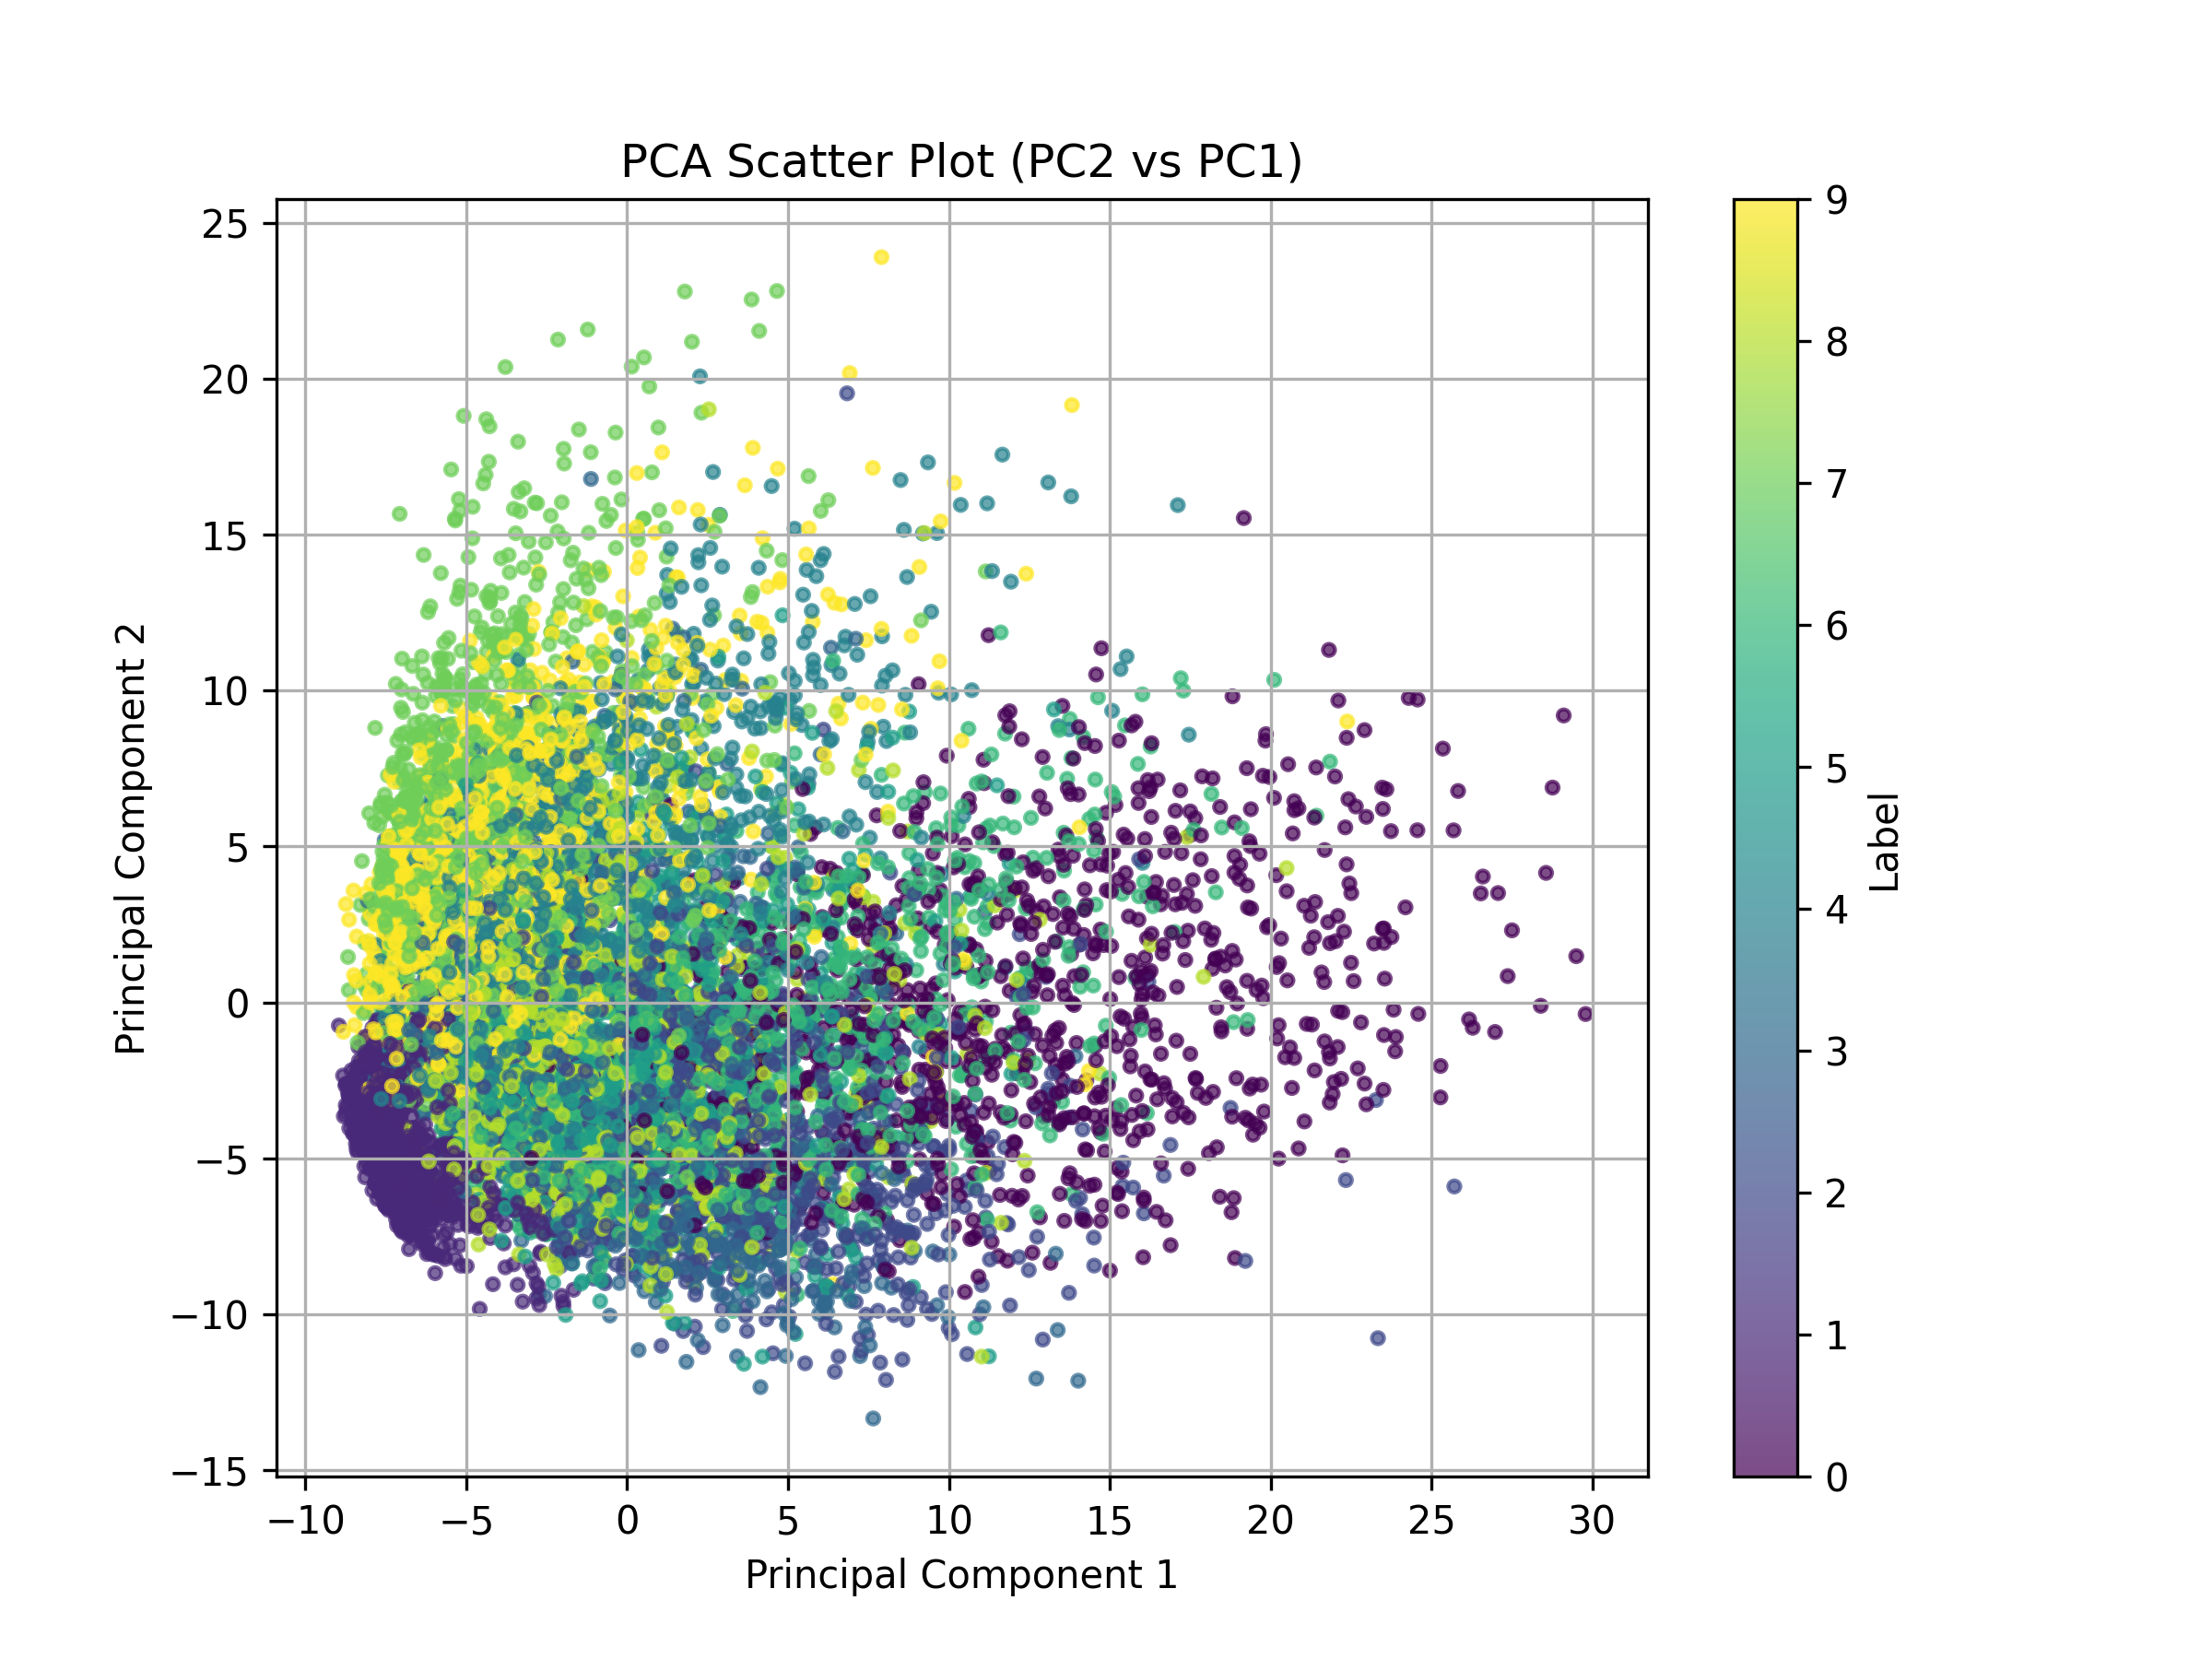
\includegraphics[width=0.6\textwidth]{Images/P3-pca_scatter_plot.png}
    \caption{PCA Scatter Plot (PC2 vs PC1)}
    \label{fig:pca_scatter_plot}
\end{figure}

\subsubsection{t-SNE Implementation}
t-SNE is applied to visualize the high-dimensional MNIST dataset in two dimensions. The following code snippet demonstrates this process:

\begin{lstlisting}[language=Python]
tsne = TSNE(n_components=2, random_state=42)
X_tsne = tsne.fit_transform(X_scaled)
\end{lstlisting}

The t-SNE scatter plot is shown in Figure \ref{fig:tsne_scatter_plot}.

\begin{figure}[H]
    \centering
    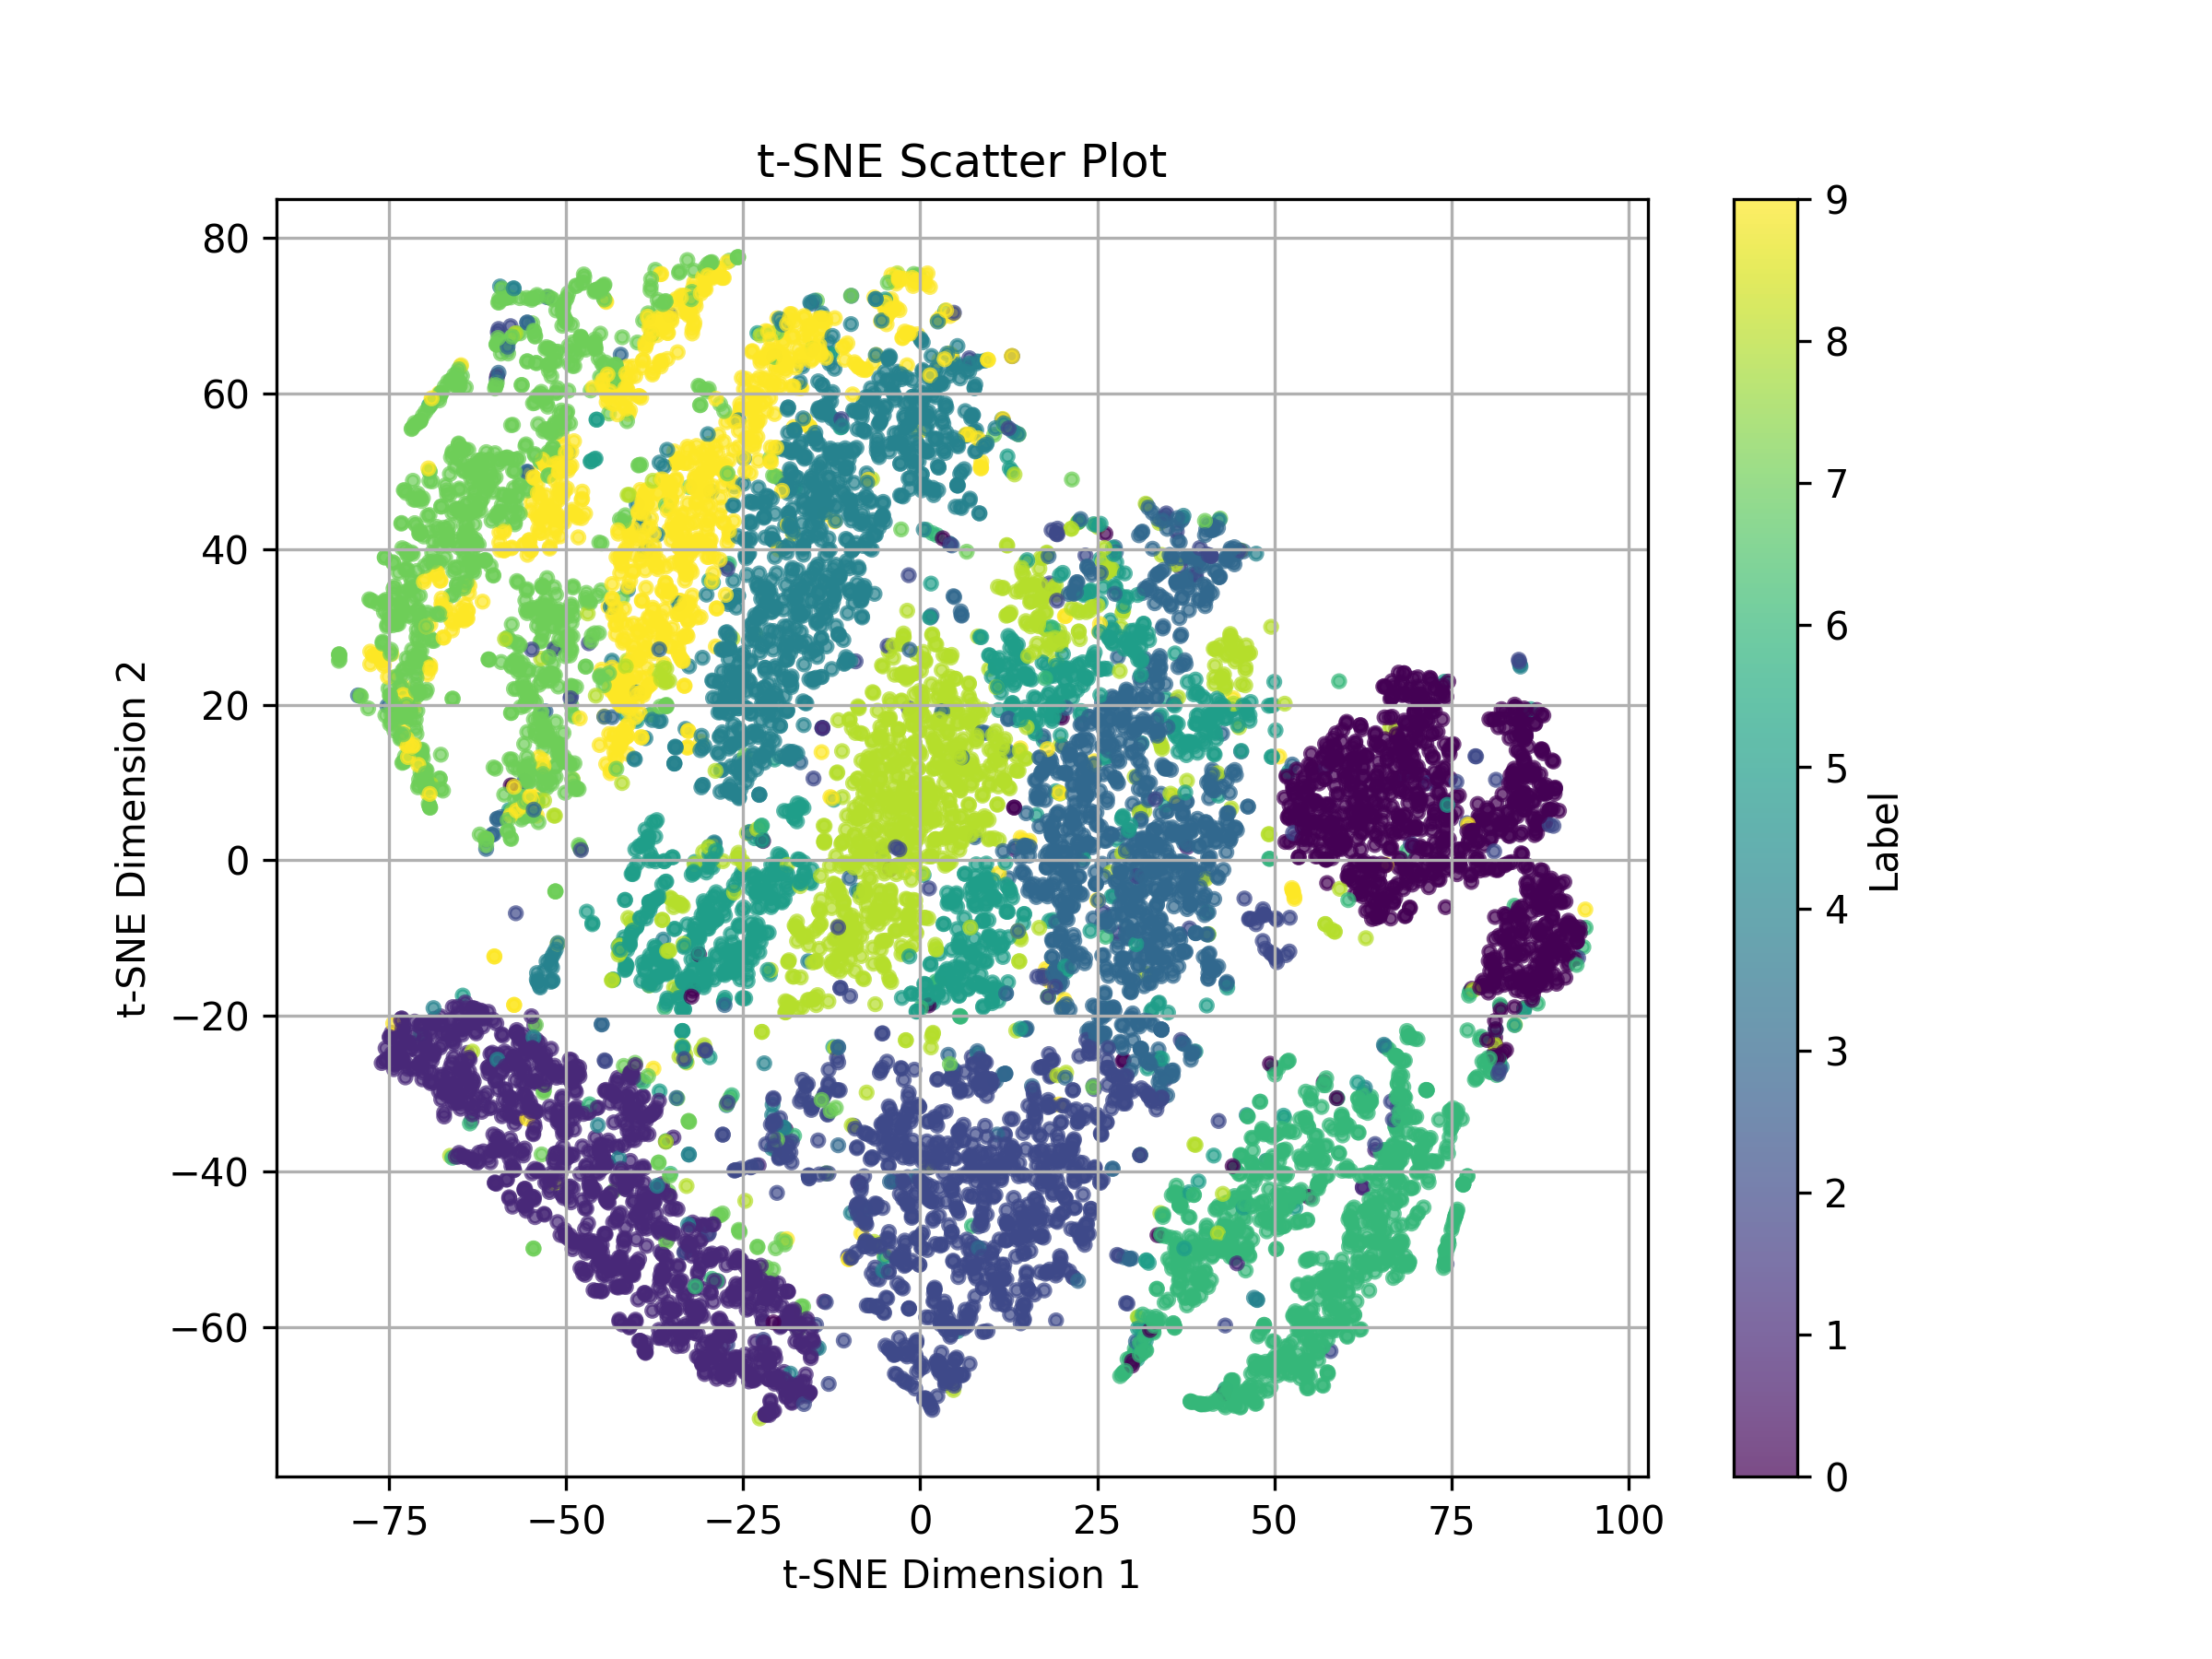
\includegraphics[width=0.6\textwidth]{Images/P3-tsne_scatter_plot.png}
    \caption{t-SNE Scatter Plot for MNIST Dataset}
    \label{fig:tsne_scatter_plot}
\end{figure}

Similarly, t-SNE is applied to the e6 dataset, and the resulting scatter plot is shown in Figure \ref{fig:tsne_scatter_plot_e6}.

\begin{figure}[H]
    \centering
    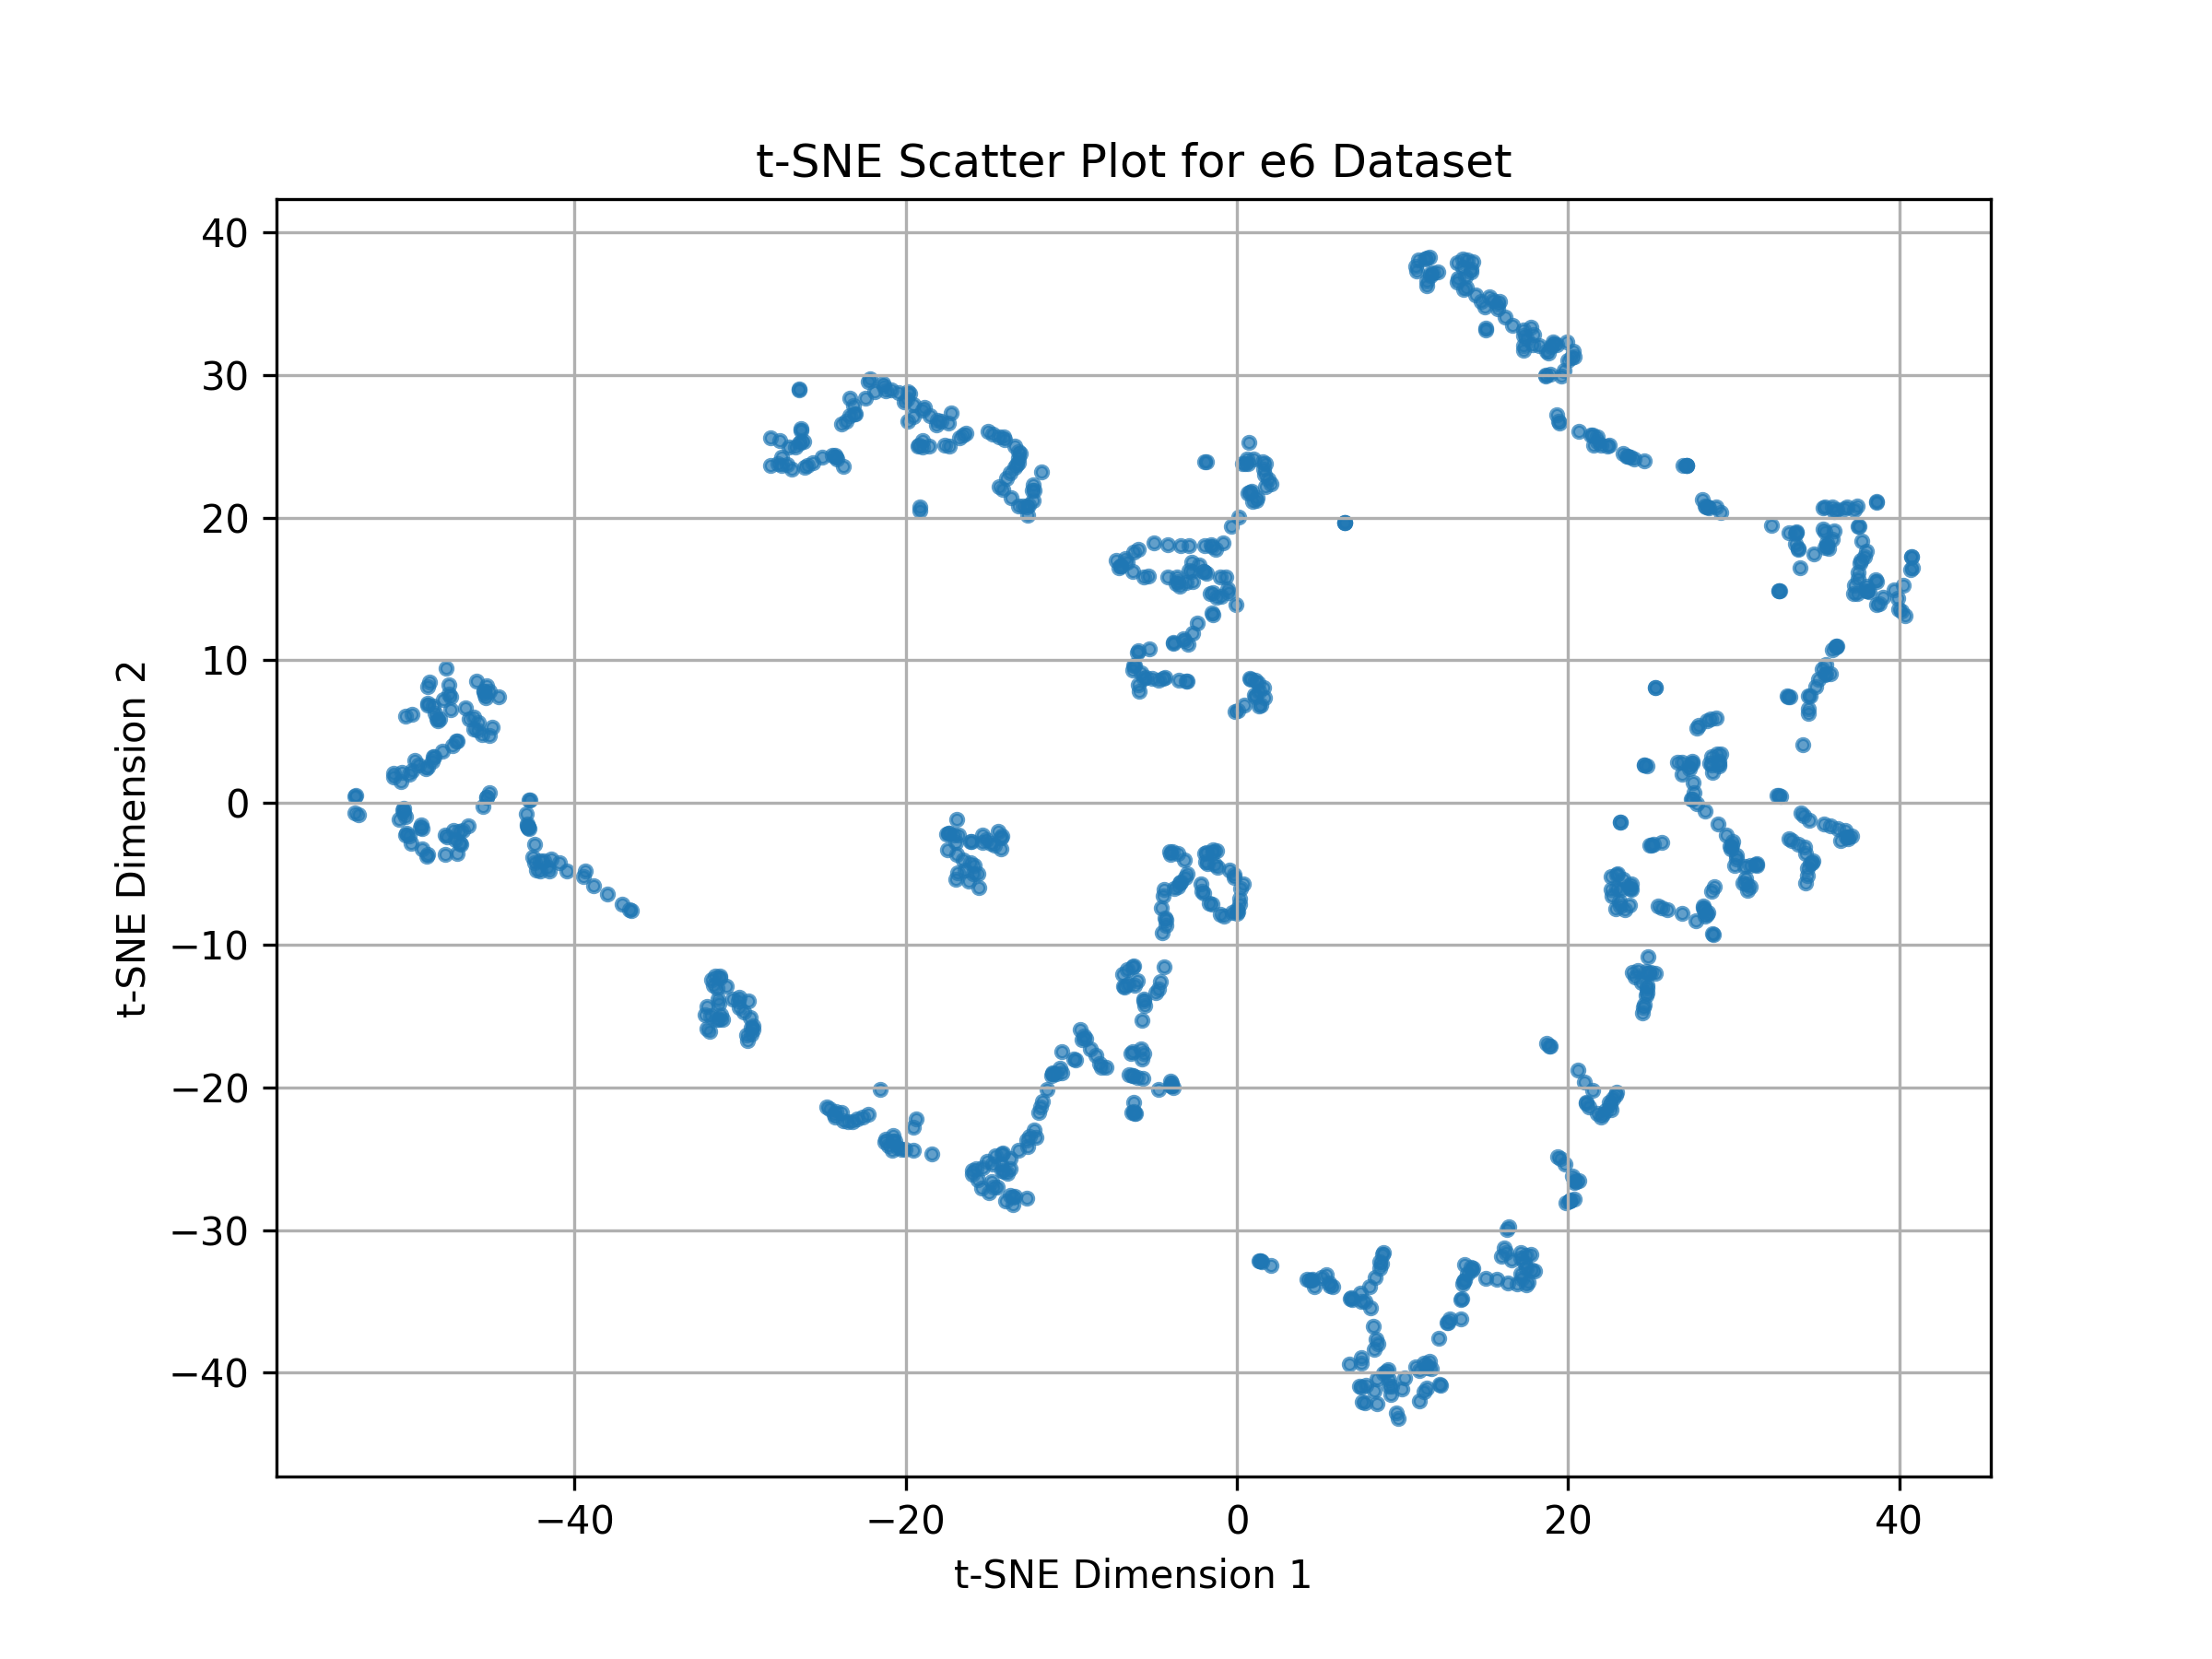
\includegraphics[width=0.8\textwidth]{Images/P3-tsne_scatter_plot_e6.png}
    \caption{t-SNE Scatter Plot for e6 Dataset}
    \label{fig:tsne_scatter_plot_e6}
\end{figure}

\subsection{Analysis and Insights}
The elbow diagram allows us to determine the optimal number of principal components for PCA by identifying the 'elbow' point, which indicates a suitable number of components to retain while preserving variance. The scatter plots provide visual insights into the distribution of the data, helping to identify clusters and separations between different classes.

PCA effectively retains the global structure of the data, while t-SNE emphasizes local similarities, making it particularly useful for classification problems in high-dimensional datasets.

\subsection{Conclusion}
This report demonstrates the effective application of PCA and t-SNE for dimensionality reduction and visualization of the MNIST and e6 datasets. The combination of PCA's explained variance analysis and t-SNE's visualization capabilities provides a comprehensive view of the inherent structures in the datasets, making it a valuable approach in exploratory data analysis and machine learning preprocessing workflows.